\chapter{تجهیزات پیشنهادی و برآورد هزینه}
\label{chap:cost}
%=====================================================================

\section{مأخذ برآورد}

برآوردهای این فصل بر مبنای قیمت‌های عمومی منتشرشده توسط تولیدکنندگان و گزارش‌های تحلیل بازار جهانی است و \textbf{صرفاً برای برنامه‌ریزی اولیهٔ بودجه} ارائه می‌شود؛ قیمت نهایی باید از طریق استعلام رسمی و مناقصهٔ بین‌المللی/داخلی مطابق مقررات ساماندهی خرید کالای دولتی مشخص شود. لازم به ذکر است که به‌دلیل تحریم‌های فناوری، ممکن است دسترسی مستقیم به برخی تولیدکنندگان غربی (\lr{ID Quantique}، \lr{Toshiba}) با محدودیت مواجه باشد و لازم است گزینه‌های جایگزین (تأمین از طریق کشورهای ثالث، یا توسعهٔ داخلی نمونهٔ اولیه با همکاری مراکز پژوهشی داخلی) نیز به‌موازات ارزیابی شود.

\section{هزینهٔ تجهیزات هر گره}

بر اساس داده‌های صنعتی، هزینهٔ یک زوج سامانهٔ \lr{QKD} تجاری (فرستنده و گیرنده) بسته به نسل فناوری و نرخ کلید، در بازهٔ وسیعی قرار می‌گیرد: نمونه‌های اولیهٔ تجاری در حدود $82000$ دلار برای یک زوج \Cite{mittech2009}، سامانه‌های میان‌رده در بازهٔ $150000$ تا $400000$ دلار \Cite{arxiv0905report}، و آشکارسازهای فوق‌پیشرفتهٔ نانوسیم ابررسانا برای برد بلند در حدود $100000$ یورو برای هر واحد \Cite{techtimes2026sweden}. برای یک شبکهٔ متروپلیتن سازمانی متوسط با دو تا سه سایت در شعاع $50$ کیلومتری، هزینهٔ کل معمولاً بین $500000$ تا $3$ میلیون دلار برآورد می‌شود \Cite{marketintelo2026}.

\begin{table}[htbp]
\centering
\caption{برآورد هزینهٔ اجزای اصلی طرح پایلوت تهران (شش گره، توپولوژی حلقه‌ای)}
\label{tab:cost}
\small
\begin{tabular}{p{5.5cm}p{3.5cm}p{4.5cm}}
\toprule
\textbf{قلم هزینه} & \textbf{برآورد (میلیون دلار)} & \textbf{توضیح} \\
\midrule
سامانه‌های \lr{QKD} (شش زوج فرستنده/گیرنده) & $1.8$ تا $3.2$ & بر مبنای سامانهٔ میان‌رده تا پیشرفته \Cite{idq2025cerberis,toshiba2026qkd} \\
\lr{KMS} و نرم‌افزار مدیریت کلید & $0.3$ تا $0.5$ & شامل مجوز نرم‌افزار و یکپارچه‌سازی \lr{API} \\
فیبر تاریک (اجاره/حفاری تکمیلی) & $0.5$ تا $0.9$ & بسته به میزان فیبر موجود مخابرات ایران \\
رمزگذارهای خط و تجهیزات شبکه & $0.4$ تا $0.8$ & رمزگذار \lr{AES-256} سازگار با \lr{QKD} \\
یکپارچه‌سازی \lr{PQC} در نرم‌افزار بانکی & $0.3$ تا $0.6$ & پیاده‌سازی \lr{ML-KEM/ML-DSA} در زیرساخت پیام‌رسانی بانکی \\
آموزش، ممیزی امنیتی و گواهی‌دهی & $0.2$ تا $0.4$ & شامل آزمون نفوذ و ارزیابی مستقل \\
بهره‌برداری و نگهداشت سالانه (سال اول) & $0.3$ تا $0.5$ & پشتیبانی فنی، پایش و به‌روزرسانی \\
\midrule
\textbf{جمع کل برآوردی (فاز پایلوت)} & \textbf{$3.8$ تا $6.9$} & \\
\bottomrule
\end{tabular}
\end{table}

شکل \ref{fig:costchart} توزیع تقریبی این هزینه‌ها را برای سناریوی میانی نشان می‌دهد.

\begin{figure}[htbp]
\centering
\begin{tikzpicture}
\begin{axis}[
  ybar,
  bar width=16pt,
  width=12.5cm,height=6.5cm,
  symbolic x coords={تجهیزات \lr{QKD},\lr{KMS},فیبر,رمزگذار,\lr{PQC},آموزش,بهره‌برداری},
  xtick=data,
  x tick label style={font=\scriptsize,rotate=20,anchor=east},
  ylabel={میلیون دلار},
  nodes near coords,
  nodes near coords style={font=\scriptsize},
  ymin=0,
  ymajorgrids=true,
  grid style=dashed,
]
\addplot[fill=blue!35] coordinates {
  (تجهیزات \lr{QKD},2.5) (\lr{KMS},0.4) (فیبر,0.7) (رمزگذار,0.6) (\lr{PQC},0.45) (آموزش,0.3) (بهره‌برداری,0.4)
};
\end{axis}
\end{tikzpicture}
\caption{توزیع تقریبی برآورد هزینهٔ فاز پایلوت (سناریوی میانی)}
\label{fig:costchart}
\end{figure}

برای مشاهدهٔ سریع‌تر سهم نسبی هر قلم هزینه از کل بودجه، شکل \ref{fig:costpie} همان داده‌ها را به‌صورت نمودار دایره‌ای نمایش می‌دهد؛ همان‌طور که مشخص است، تنها تجهیزات \lr{QKD} به‌تنهایی نزدیک به نیمی از کل بودجهٔ فاز پایلوت را تشکیل می‌دهد.

\begin{figure}[htbp]
\centering
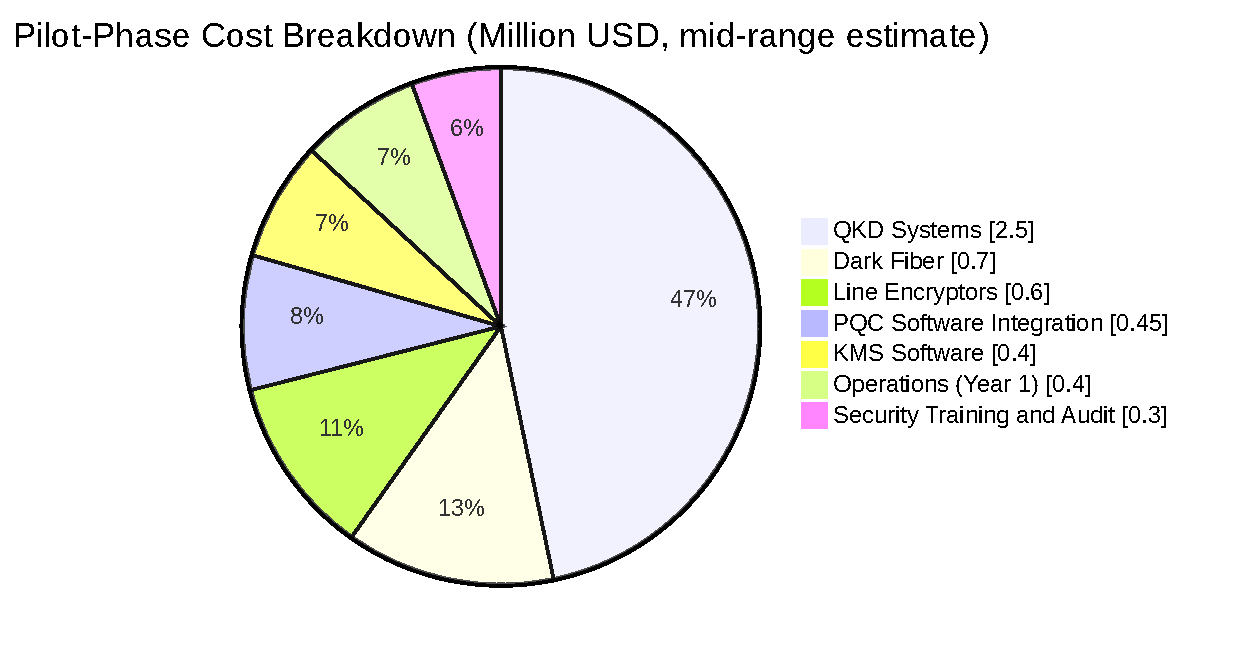
\includegraphics[width=0.72\linewidth]{figs/fig_cost_pie.pdf}
\caption{سهم نسبی هر قلم از برآورد هزینهٔ فاز پایلوت}
\label{fig:costpie}
\end{figure}

\section{فهرست تجهیزات آزمایشگاهی و قطعات الکترونیکی}
\label{sec:labequipment}

جدول \ref{tab:cost} تصویری از هزینهٔ کلان یک سامانهٔ \lr{QKD} «تجاری و آمادهٔ‌نصب» را نشان می‌دهد، اما واقعیت این است که هیچ تیم مهندسی جدی نباید صرفاً به خرید یک محصول بستهٔ خارجی بسنده کند. پیش از هر تصمیم خرید بزرگ، تیم پروژه به یک آزمایشگاه داخلی نیاز دارد تا بتواند پروتکل انتخابی (مثلاً \lr{decoy-state BB84} یا نسخهٔ ترکیبی \lr{TF-QKD-McEliece} معرفی‌شده در فصل \ref{chap:hybrid}) را روی میز کار خودش پیاده‌سازی، کالیبره و آزمون کند، رمزگشای \lr{LDPC} را روی سخت‌افزار واقعی سنجش‌پذیری بدهد و پیش از هر تعهد مالی بزرگ، دانش فنی لازم برای مذاکرهٔ آگاهانه با تأمین‌کنندگان را در داخل کشور انباشته کند. جدول \ref{tab:labgear} فهرستی از مهم‌ترین اقلام مورد نیاز این آزمایشگاه را ارائه می‌دهد؛ برای اقلامی که به‌صورت واقعی در بازار داخلی (سایت \lr{ترب}) قابل استعلام بودند، قیمت واقعی به‌همراه پانویس منبع آورده شده است، و برای اقلام تخصصیِ فوتونیک/کوانتومی که در بازار عمومی داخلی یافت نشدند، این موضوع به‌صراحت قید شده است.

 	\begin{longtable}{p{4cm}p{3.2cm}p{6.3cm}}
 		\caption{فهرست تجهیزات آزمایشگاهی پیشنهادی برای فاز تحقیق و توسعه}
 		\label{tab:labgear} \\
 		\toprule
 		\textbf{قلم} & \textbf{کاربرد در پروژه} & \textbf{برآورد قیمت و وضعیت تأمین} \\
 		\midrule
 		\endfirsthead
 		
 		\caption[]{فهرست تجهیزات آزمایشگاهی پیشنهادی برای فاز تحقیق و توسعه (ادامه)} \\
 		\toprule
 		\textbf{قلم} & \textbf{کاربرد در پروژه} & \textbf{برآورد قیمت و وضعیت تأمین} \\
 		\midrule
 		\endhead
 		
 		\midrule
 		\endfoot
 		
 		\bottomrule
 		\endlastfoot
 		
 		\small
 		برد توسعهٔ \lr{FPGA} (رده \lr{Artix-7}/\lr{Spartan-6})\footnote{به‌عنوان نمونه، نمونه‌های \lr{Xilinx Spartan-6 XC6SLX9} و \lr{Artix-7} در بازار داخلی از طریق فروشگاه‌های آنلاین قابل استعلام‌اند، ر.ک. \url{https://torob.com/p/760564e7-1a4b-435c-854b-ca885dfdc4cb/} و \url{https://torob.com/p/bf1b3599-8467-4ed5-a232-2b44103b5a4f/}.} & پیاده‌سازی رمزگشای \lr{QC-/SC-LDPC}، منطق زمان‌بندی آشکارسازی فوتون و رابط \lr{McEliece} & حدود $4$ تا $22$ میلیون تومان برای رده‌های آموزشی/میان‌رده (کاملاً در دسترس داخل کشور)؛ رده‌های پیشرفته‌تر (\lr{Kintex}/\lr{UltraScale}) به دلیل ساخت شرکت آمریکایی \lr{AMD/Xilinx} در فهرست کنترل صادرات قرار دارند \\
 		اسیلوسکوپ/تحلیل‌گر زمانی پهن‌باند (رده \lr{GHz})\footnote{اسیلوسکوپ‌های آموزشی و صنعتی رده مگاهرتزی به‌وفور و ارزان در بازار داخلی موجودند، برای نمونه ر.ک. \url{https://torob.com/p/ec33ce7c-90e0-435e-b53e-e7a15e031d09/}؛ اما رده \lr{GHz} لازم برای اندازه‌گیری \lr{jitter} آشکارساز تک‌فوتون در این جست‌وجو یافت نشد.} & اندازه‌گیری دقیق زمان رسیدن فوتون و \lr{jitter} آشکارساز برای برآورد \lr{QBER} & رده‌های عمومی مگاهرتزی حدود $2$ تا $4$ میلیون تومان (در دسترس داخل)؛ رده \lr{GHz} تجهیز آزمایشگاهی تخصصی \lr{Keysight/Tektronix} است که به‌طور معمول در بازار عمومی داخلی عرضه نمی‌شود \\
 		ماژول لیزر پالسی تک‌طول‌موج \lr{1550nm} (منبع فوتون ضعیف‌شده) & تولید حالت‌های کوانتومی نور برای پروتکل \lr{QKD} در پنجرهٔ مخابراتی کم‌تلفات & در جست‌وجوی بازار داخلی یافت نشد؛ تأمین‌کنندگان اصلی عمدتاً شرکت‌های چینی فعال در حوزهٔ فیبر نوری‌اند، مسیر تأمین قابل‌اجرا اما با زمان تحویل چندهفته‌ای \\
 		آشکارساز تک‌فوتون (\lr{SPAD} یا \lr{SNSPD}) & هستهٔ دریافت سیگنال کوانتومی در گیرندهٔ \lr{QKD}؛ حساس‌ترین و گران‌ترین جزء کل سامانه & \textbf{پرریسک‌ترین قلم از منظر تحریم}: تولیدکنندگان اصلی (\lr{ID Quantique}، \lr{Single Quantum}، \lr{Photon Spot}) آمریکایی/اروپایی‌اند و این رده از آشکارساز به‌طور مشخص در فهرست‌های کنترل صادرات فناوری کوانتومی قرار می‌گیرد؛ مسیر پیشنهادی، سرمایه‌گذاری موازی روی توسعهٔ داخلی نمونهٔ اولیه با مشارکت گروه‌های پژوهشی اپتوالکترونیک دانشگاهی کشور است \\
 		مدولاتور فاز/دامنهٔ نوری (لیتیوم‌نایوبات) و کنترل‌کنندهٔ پلاریزاسیون & کدگذاری بیت کوانتومی در پایه \lr{X}/\lr{Z} و همسوسازی قطبش نور فرستنده و گیرنده & قطعهٔ فوتونیک تخصصی (عمدتاً \lr{Thorlabs}، \lr{iXblue})؛ در بازار داخلی یافت نشد، نیازمند تأمین بین‌المللی \\
 		ژنراتور اعداد تصادفی کوانتومی (\lr{QRNG}) سخت‌افزاری & تولید بیت‌های تصادفی حقیقی برای انتخاب پایه و فاز در پروتکل \lr{QKD} و همچنین کلیدسازی \lr{PQC} & همان دستهٔ تحریمی سامانه‌های \lr{QKD} کامل (بخش \ref{sec:pqcfoundations})؛ در نبود امکان خرید مستقیم، پیاده‌سازی نرم‌افزاری مبتنی بر \lr{TRNG} تأییدشدهٔ داخلی جایگزین موقت قابل‌قبولی است \\
 		ماژول امنیت سخت‌افزاری (\lr{HSM}) سازگار با \lr{PQC} & نگهداری امن کلیدهای \lr{ML-KEM/ML-DSA} در زیرساخت بانکی & تجهیز رمزنگاری تحت کنترل صادرات (چارچوب \lr{Wassenaar})؛ عمدتاً \lr{Thales}/\lr{Utimaco}؛ گزینهٔ جایگزین، توسعهٔ \lr{HSM} نرم‌افزاری/داخلی با گواهی امنیتی داخلی است \\
 		رک سرور، سوئیچ شبکه و منبع تغذیهٔ بی‌وقفه (\lr{UPS}) & زیرساخت عمومی محاسباتی و شبکه برای \lr{KMS} و سرورهای رمزگذاری & تجهیز استاندارد \lr{IT}، به‌طور کامل و با تنوع زیاد در بازار داخلی موجود و بدون ملاحظهٔ تحریمی خاص \\
 	\end{longtable}


نکتهٔ مهمی که از این جدول برمی‌آید این است که ریسک تحریم به‌هیچ‌وجه یکنواخت پخش نشده است: قطعات دیجیتال و محاسباتی عمومی (برد \lr{FPGA} رده میانی، سرور، شبکه) به‌سادگی و با قیمت مقرون‌به‌صرفه در بازار داخلی قابل تهیه‌اند، در حالی که قلب فیزیکی سامانهٔ \lr{QKD}، یعنی منبع فوتون، آشکارساز تک‌فوتون و مدولاتور نوری، دقیقاً همان اجزائی هستند که به‌دلیل ماهیت دوکاربردی (\lr{dual-use}) فناوری کوانتومی، سخت‌ترین محدودیت‌های صادراتی را تجربه می‌کنند. به همین دلیل، در فصل \ref{chap:roadmap} فاز تدارکات این اقلام حساس عمداً زودتر از موعد و به‌موازات فازهای طراحی آغاز می‌شود، نه پس از اتمام آن‌ها، چرا که هرگونه تأخیر در تأمین همین چند قلم است که مستقیماً کل زمان‌بندی طرح را تعیین می‌کند، نه پیچیدگی مهندسی نرم‌افزار یا پروتکل.

\section{برآورد نیروی انسانی و بودجهٔ جبران خدمت}
\label{sec:humanresources}

فارغ از تجهیزات، مهم‌ترین منبعی که این طرح به آن نیاز دارد، تیمی است که بتواند هم‌زمان زبان فیزیک کوانتوم، رمزنگاری پساکوانتومی، طراحی سخت‌افزار و یکپارچه‌سازی سامانه‌های بانکی را بفهمد، ترکیبی که به‌ندرت در یک نفر جمع می‌شود و لذا باید از دل یک تیم چندتخصصی بیرون بیاید. جدول \ref{tab:hr} ترکیب پیشنهادی این تیم را برای فاز پایلوت (افق $12$ تا $18$ ماهه، مطابق فصل \ref{chap:roadmap}) نشان می‌دهد. سطح حقوق پیشنهادی بر مبنای بازهٔ رایج بازار کار فناوری اطلاعات و امنیت سایبری کشور در نظر گرفته شده، از حدود $30$ میلیون تومان برای سطح جونیور تا حدود $200$ میلیون تومان برای سطح سینیور/متخصص ارشد، و طبیعتاً باید در زمان اجرای واقعی طرح با نرخ روز بازار و مصوبات سازمان امور استخدامی کشور تطبیق داده شود.

\begin{table}[htbp]
\centering
\caption{ترکیب پیشنهادی نیروی انسانی هستهٔ فاز پایلوت}
\label{tab:hr}
\small
\begin{tabular}{p{4.3cm}p{2.1cm}p{2.6cm}p{1.3cm}p{2.4cm}}
\toprule
\textbf{نقش} & \textbf{سطح} & \textbf{حقوق ماهانه (میلیون تومان)} & \textbf{تعداد} & \textbf{جمع ماهانه (میلیون تومان)} \\
\midrule
مدیر پروژه & سینیور & $190$ & $1$ & $190$ \\
مهندس فیزیک/پروتکل \lr{QKD} & سینیور & $170$ & $2$ & $340$ \\
مهندس سخت‌افزار/\lr{FPGA} & میان‌رده & $100$ & $2$ & $200$ \\
مهندس نرم‌افزار رمزنگاری \lr{PQC} & میان‌رده تا سینیور & $110$ & $2$ & $220$ \\
مهندس شبکه و فیبر نوری & میان‌رده & $75$ & $2$ & $150$ \\
کارشناس امنیت سایبری و ممیزی نفوذ & سینیور & $140$ & $1$ & $140$ \\
توسعه‌دهندهٔ یکپارچه‌سازی بانکی (\lr{API}/میان‌افزار) & میان‌رده & $85$ & $2$ & $170$ \\
تکنسین آزمایشگاه اپتیک و نصب میدانی & جونیور تا میان‌رده & $40$ & $2$ & $80$ \\
کارشناس تدارکات، امور گمرکی و حقوقی & میان‌رده & $65$ & $1$ & $65$ \\
کارشناس مستندسازی و کنترل کیفیت & جونیور & $38$ & $1$ & $38$ \\
\midrule
\textbf{جمع کل تیم هسته ($16$ نفر)} & & & & \textbf{$\approx 1{,}593$} \\
\bottomrule
\end{tabular}
\end{table}

با این ترکیب، هزینهٔ ماهانهٔ نیروی انسانی هستهٔ طرح در حدود $1.6$ میلیارد تومان و هزینهٔ سالانهٔ آن در حدود $19$ میلیارد تومان برآورد می‌شود؛ این رقم عمداً جدا از جدول \ref{tab:cost} (که تنها هزینهٔ تجهیزات و یکپارچه‌سازی است) نگه داشته شده تا در بودجه‌ریزی نهایی، ردیف «نیروی انسانی» به‌عنوان یک قلم مستقل و قابل‌ردیابی از ردیف «سرمایه‌ای/تجهیزاتی» دیده شود، تفکیکی که معمولاً در مصوبات بودجهٔ دستگاه‌های دولتی نیز الزامی است. بدیهی است دو نقش نخست جدول، یعنی مهندس ارشد فیزیک/پروتکل \lr{QKD} و مدیر پروژه، کمیاب‌ترین و در عین حال حیاتی‌ترین حلقهٔ این زنجیره‌اند؛ پیشنهاد می‌شود جذب این دو نقش، حتی پیش از قطعی‌شدن بودجهٔ کامل طرح، در اولویت نخست قرار گیرد.



بازار جهانی \lr{QKD} در افق سال $2035$ به حدود $20$ میلیارد دلار برآورد می‌شود \Cite{toshiba2020launch}. توسعهٔ طرح از مقیاس پایلوت کلان‌شهری به یک کریدور بین‌شهری (مثلاً تهران-اصفهان یا تهران-مشهد) نیازمند سرمایه‌گذاری در مقیاس ده‌ها میلیون دلار و افق زمانی چندساله خواهد بود و پیشنهاد می‌شود صرفاً پس از تکمیل موفق و ارزیابی امنیتی فاز پایلوت بررسی شود.

%=====================================================================
